\chapter{Contextualização}

O objetivo deste capítulo é fornecer subsídios para a compreensão dos assuntos tratados nesta dissertação. Primeiramente, contextualiza-se o paradigma
de Programação Orientada a Aspectos (POA), apresentando a motivação para o uso de aspectos e as construções específicas da linguagem AspectJ, que devem ser representáveis 
na modelagem. A segunda parte discorre sobre a análise e projeto de sistemas utilizando a segunda versão da UML. Apresentam-se alguns conceitos sobre
análise e projeto e os diagramas da UML. O tópico final fala sobre meta-modelagem, que permite estender um modelo para representar elementos de um
domínio específico.

\section{Programação Orientada a Aspectos}

Esta seção discorre sobre a separação de um sistema em um conjunto de interesses e os problemas decorrentes da implementação de interesses com os
paradigmas tradicionais. Devido a estes problemas, surge a necessidade de um novo paradigma para realizar a separação de interesses: o paradigma de
Programação Orientada a Aspectos (POA). A seção é finalizada com a apresentação da principal linguagem para implementação de aspectos em Java: 
AspectJ.

\subsection{Abstração de Interesses}\label{sec:concerns_abstraction}

Ao iniciar a análise e projeto de um sistema, existe um conjunto de requisitos que devem ser implementados para satisfazer as necessidades do cliente.
Cada requisito pode ser considerado um interesse que deve ser realizado para finalizar o sistema como um todo. Assim, um sistema é composto por um
conjunto de interesses. Em um sistema para gerenciamento de hotel, por exemplo, é possível identificá-los como: reserva de quartos, \textit{check-in},
\textit{check-out}, acúmulo de pontos em um programa de fidelidade, controle de uma lista de espera, registro de mensagens, controle de acesso,
garantia de \textit{performance}, etc \cite{Jacobson:2004:ASD:1062430}.

\begin{figure}[!hb]
	\centering
	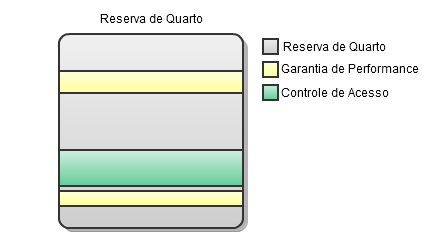
\includegraphics{img/context_aspect_concerns.png}
	\caption{Separação de interesses do módulo para reserva de quarto}\label{fig:context_aspect_concerns}
\end{figure}

No sistema de gerenciamento de hotel, é possível classificar reserva de quartos, \textit{check-in} e \textit{check-out} como interesses núcleo.
Os interesses de controle de acesso, acúmulo de pontos em um programa de fidelidade, controle de uma lista de espera, registro de mensagens e garantia
de \textit{performance} impactam diversas partes do sistema, por isso, são classificados como interesses entrecortantes. O interesse de controle de acesso deve 
verificar quais usuários podem acessar quais partes do sistema e, por isso, deve ser executado em todos os interesses núcleo. O interesse de
acúmulo de pontos em um programa de fidelidade impacta qualquer pagamento realizado. O interesse de controle de uma lista de espera impacta a
reserva de quartos. Já o registro de mensagens impacta grande parte dos interesses, pois as transações do sistema são registradas. Garantia de
\textit{performance} impacta todos os outros interesses, pois para garantir \textit{peformance} todo o sistema deve ser implementado com restrições
de segurança.

Utilizando os paradigmas convencionais para implementação de interesses, como a Programação Orientada a Objetos (POO), o módulo
para implementar o interesse de reserva de quartos seria composto  por código referente a reserva, e também a garantia de \textit{performance} e 
controle de acesso. A figura \ref{fig:context_aspect_concerns} mostra os interesses presentes no módulo de reserva de quartos. Observa-se a
implementação de vários interesses no mesmo módulo. Segundo Laddad\cite{Laddad:2003:AAP:993468}, essa situação é conhecida como \textbf{emaranhamento
de código} (\textit{code tangling}).

Outro sintoma de implementação deselegante de interesses é o \textbf{espalhamento de código} (\textit{code scattering}), quando o código 
referente a um mesmo interesse está disposto em diferentes módulos \cite{Laddad:2003:AAP:993468}. O espalhamento de código pode acontecer em duas
situações:

\begin{itemize}
  \item \textbf{Duplicação de código}: Diferentes módulos núcleo executam código
  referente a um mesmo interesse entrecortante.  
  
  Exemplo: Interesse para registro de informações (\textit{logging}) de um
  sistema; cada módulo núcleo contém chamadas a métodos da API
  de \textit{logging} para registrar informações.
  
  \item \textbf{Complementação de código}: Diferentes módulos executam código
  complementar para implementar um interesse entrecortante. 
  
  Exemplo: Interesse para autorização em um sistema; um módulo implementa o
  gerenciamento da sessão, outro módulo implementa o gerenciamento de
  permissões e controle de acesso e outro realiza a autenticação de usuários;
  cada módulo implementa uma parte do interesse de autorização.
\end{itemize}

O emaranhamento e espalhamento de código dificultam a manutenção de um sistema,
pois modificar um interesse impacta em modificar diferentes módulos. Além
disso, é complicado realizar um rastreamento entre interesses e módulos, pois o
código de um interesse está disposto em mais de um módulo. Outro problema é a
dificuldade de reuso de módulos devido a dependência de um módulo com vários
interesses \cite{Laddad:2003:AAP:993468}. 

\subsection{A necessidade de aspectos}

Os problemas destacados na sessão \ref{sec:concerns_abstraction} indicam a
necessidade de separação de interesses em diferentes módulos. A Programação Orientada a Aspectos 
(POA) \cite{Kiczales97aspect-orientedprogramming} é um paradigma de programação para representar
elegantemente os interesses de um sistema que impactam diversos módulos. 
Uma representação elegante de um interesse o separa em um único módulo e permite
o reuso entre diferentes aplicações. O objetivo da POA é a modularização dos interesses entrecortantes 
para que os mesmos fiquem separados dos módulos que implementam os interesses
núcleo da aplicação \cite{Laddad:2003:AAP:993468}.

É importante observar que, boa parte dos interesses de uma aplicação
são interesses núcleo e podem ser implementados elegantemente com a POO. Por
isso, a POA não pretende substituir a Programação Orientada a Objetos (POO), 
mas sim complementá-la com uma melhor representação para os interesses
entrecortantes.

\subsection{Metodologia de desenvolvimento}

Segundo \cite{Laddad:2003:AAP:993468}, para implementar um sistema utilizando aspectos
geralmente executam-se três fases:


\begin{enumerate}
  \item \textbf{Decomposição de Aspectos}: Identificação de quais requisitos são
  interesses núcleo e quais são interesses entrecortantes.
  \item \textbf{Implementação de Interesses}: Implementação de cada interesse
  separadamente.
  \item \textbf{Composição de Aspectos} (\textit{Weaving}): É a implementação de
  um aspecto para cada interesse entrecortante. O aspecto define o comportamento
  que será executado em determinados pontos de execução de um ou mais interesses. 
  Cada interesse entrecortante está contido em um único módulo: o aspecto. Após
  a implementação dos aspectos, se inicia o processo de composição \textit{weaving} 
  que insere o comportamento dos interesses entrecortantes nos interesses núcleo
  (nos pontos definidos nos aspectos). A figura \ref{fig:aspects_weaving} mostra
  o fluxo de desenvolvimento de uma aplicação orientada a aspectos.
\end{enumerate}

\begin{figure}[!hb]
	\centering
	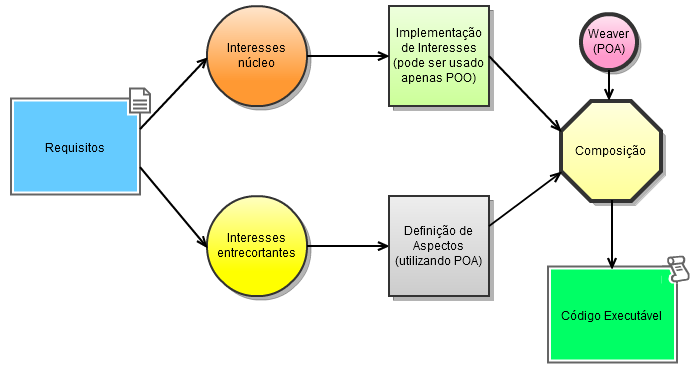
\includegraphics[scale=0.6]{img/aspects_weaving.png}
	\caption{Fluxo de desenvolvimento de uma aplicação com aspectos}\label{fig:aspects_weaving}
\end{figure}

\subsection{A linguagem AspectJ}

A linguagem AspectJ \cite{AspectJ11} é uma extensão da linguagem Java para programação orientada a aspectos. Qualquer programa implementado em Java
pode ser estendido utilizando AspectJ. A linguagem provê mecanismos para representar interesses entrecortantes e permite a composição dos mesmos com os interesses 
núcleo de um sistema. A linguagem oferece construções de extensão comportamentais e estáticas. As extensões comportamentais permitem que um novo
comportamento seja executado antes, durante ou depois de um determinado ponto de execução do sistema. As extensões estáticas permitem adicionar novos elementos na
estrutura das classes, por exemplo, a inserção de um novo método ou atributo. O conteúdo das próximas seções é baseado no guia de programação da
linguagem AspectJ \cite{aspectjguide} e no livro AspectJ: in Action \cite{Laddad:2003:AAP:993468}. Os exemplos, no entanto, são originais desta
dissertação.

\subsubsection{Construções Comportamentais}

Um dos principais conceitos comportamentais que devem ser compreendidos na linguagem é o de \textbf{ponto de junção}. Um ponto de junção é um
determinado ponto na execução de um programa. É importante observar que, um ponto de junção não é uma construção sintática de AspectJ, mas sim um conceito. 

A figura \ref{fig:aspects_join_point_model} descreve o fluxo de execução de um programa através da troca de mensagens entre diferentes objetos. Nesta
troca de mensagens existem diversos pontos de junção que podem ser capturados pela linguagem AspectJ. A seguir, será destacado cada ponto de junção
nesse fluxo de execução. No início da troca de mensagens, é chamado o método \textbf{umMetodo()} do \textbf{objetoA}. A chamada de um método em
AspectJ é representada pelo ponto de junção \textit{call}. Após a chamada do método, o código do mesmo será executado. A execução de um método é
representada pelo ponto de junção \textit{execution}. A duração de execução do método \textbf{umMetodo()} pode ser visualizada na ocorrência de
execução em azul. No início da execução de \textbf{umMetodo()}, realiza-se a chamada a \textbf{outroMetodo()}. A ocorrência de execução em verde
representa a duração da execução desse método. Dentro de \textbf{outroMetodo()} o método \textbf{metodoInterno()} é chamado. A ocorrência de execução em 
amarelo representa a duração de sua execução. Finalmente, instancia-se o \textbf{objetoC} através da chamada \textit{new}. A chamada de um construtor
também é um ponto de junção \textit{call} em AspectJ. A execução do mesmo pode ser capturada com o ponto de junção \textit{execution}. O tempo de
execução da instanciação desse construtor pode ser visualizado na ocorrência de execução em rosa. Os pontos de junção \textit{call} e
\textit{execution} são utilizados para capturar chamada e execução de métodos e construtores. 

\begin{figure}[!hb]
	\centering
	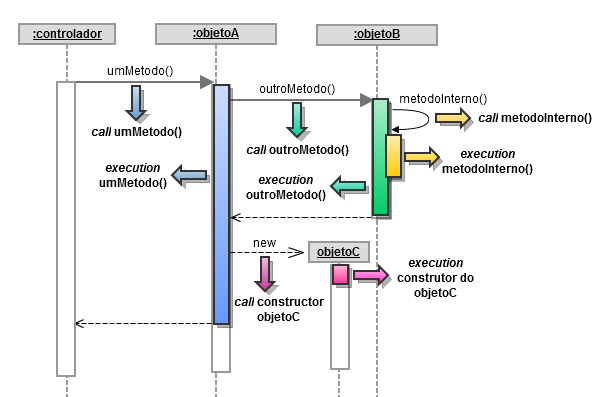
\includegraphics[scale=0.8]{img/aspects_join_point_model.png}
	\caption{Identificação de pontos de junção}\label{fig:aspects_join_point_model}
\end{figure}

É importante observar a diferença entre entre os pontos de junção de \textbf{chamada} (\textit{call}) e \textbf{execução} (\textit{execution}). Um
ponto de junção de chamada não está no código do método ou construtor sendo chamado, mas sim no código de quem está chamando o método ou construtor em
questão. Observe na figura \ref{fig:call_vs_execution} que a chamada (\textit{call}) ao método \textbf{umMetodo()} é realizada dentro do código
\textit{main} da aplicação. Já o ponto de junção de execução de um método ou construtor é disparado no corpo do método ou construtor em questão.
Observa-se na figura que a execução (\textit{execution}) do método \textbf{umMetodo()} refere-se à execução do código do próprio método.

\begin{figure}[!hb]
	\centering
	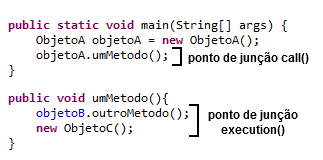
\includegraphics{img/call_vs_execution.png}
	\caption{Diferença entre os pontos de junção de chamada (call) e execução (execution)}\label{fig:call_vs_execution}
\end{figure}

O modelo de pontos de junção de AspectJ permite capturar também o tratamento de exceções, acesso e modificação de atributos (\textit{get} e
\textit{set}), inicialização e pré-inicialização de objetos, contexto de uma execução e execução de avisos. Estes pontos de junção também devem ser
representáveis em uma proposta para modelagem de programas orientados a aspectos.

Os pontos de junção em AspectJ definem quais são os pontos da execução de um programa possíveis de serem capturados. A linguagem deve disponibilizar
alguma construção sintática para selecionar pontos de junção. Para isso, AspectJ disponibiliza os \textbf{pontos de corte} (\textit{pointcuts}). Um
ponto de corte permite selecionar um conjunto de pontos de junção. 

Existem dois tipos de ponto de corte:

\begin{itemize}
  \item \textbf{Com nome}: Tem um nome e pode ser referenciado dentro de um
  aspecto.
  \item \textbf{Anônimo}: Não tem um nome e não pode ser referenciado dentro de
  um aspecto. Geralmente é definido dentro de um ponto de corte nomeado.
\end{itemize}

\begin{figure}
	\centering
	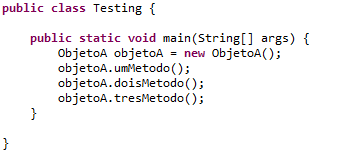
\includegraphics{img/pointcut_code.png}
	\caption{Exemplo de código em Java}\label{fig:pointcut_code}
\end{figure}

O código da figura \ref{fig:pointcut_code} mostra o exemplo de um simples código
em Java. É possível capturar pontos específicos da execução deste código
com pontos de corte. O ponto de corte \textbf{exemploDePontoDeCorte()} foi
definido para capturar chamadas ao método \textbf{umMetodo()} de objetos do tipo \textbf{ObjetoA}. 
Este ponto de corte é composto por dois pontos de corte anônimos e pode ser 
visualizado na figura \ref{fig:pointcut_vs_joinpoint}. O primeiro ponto de corte
anônimo seleciona um ponto de junção, capturando as chamadas ao método \textbf{umMetodo()} de 
objetos do tipo \textbf{ObjetoA}. O segundo ponto de corte anônimo seleciona vários
pontos de junção, pois captura qualquer chamada a membros (atributos, métodos,
construtores, etc) de objetos do tipo \textbf{ObjetoA}. 
É importante observar que, o segundo ponto de corte anônimo seleciona vários
pontos de junção em uma única definição. Entre os dois pontos de corte anônimos 
encontra-se o operador binário \textbf{\&\&}. Este operador especifica que o ponto de corte
\textbf{exemploDePontoDeCorte()} somente será satisfeito se \textbf{os dois
pontos de corte anônimos forem satisfeitos}. Assim, o ponto de corte
\textbf{exemploDePontoDeCorte()} seleciona apenas um ponto de junção: execução da
chamada ao método \textbf{umMetodo()} com o método membro de um objeto do
tipo \textbf{ObjetoA}. A captura de um único método pode ser visualizada no
código na parte inferior da figura \ref{fig:pointcut_vs_joinpoint}
(método selecionado está destacado com uma flecha laranja).

\begin{landscape}
\begin{figure*}
	\centering
	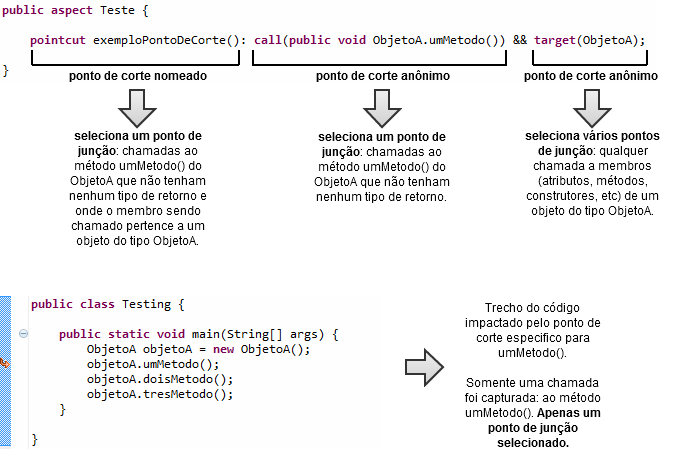
\includegraphics[scale=0.9]{img/pointcut_vs_joinpoint.png}
	\caption{Exemplo de ponto de corte}\label{fig:pointcut_vs_joinpoint}
\end{figure*}
\end{landscape}

Para possibilitar a captura de vários pontos de junção em um mesmo ponto de
corte de maneira praticável, AspectJ disponibiliza os \textbf{wildcards}. 
Um \textit{wildcard} é semelhante a uma expressão regular. As seguintes notações
estão disponíveis na definição de \textit{wildcards}:

\begin{itemize}
  \item * representa qualquer número de caracteres, exceto pontos.
  \item .. representa um ou mais caracteres, incluindo qualquer número de
  pontos.
  \item + representa uma subclasse ou sub-interface de um dado tipo.
\end{itemize}

Utilizando \textit{wildcards} é possível modificar o ponto de corte especificado na figura \ref{fig:pointcut_vs_joinpoint} para que capture chamadas
para qualquer método pertencente a objetos do tipo \textbf{ObjetoA}. Para isso, modifica-se o primeiro ponto de corte anônimo, substituindo
\textbf{umMetodo()} pela notação \textbf{*}, capturando agora todos os métodos do ObjetoA, independente do nome. Além disso, adiciona-se a 
notação \textbf{..}, capturando métodos com qualquer número de parâmetros. 

\begin{landscape}
\begin{figure*}
	\centering
	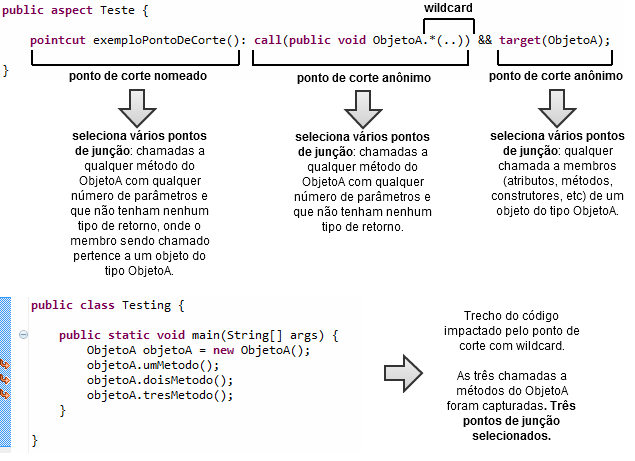
\includegraphics[scale=0.9]{img/pointcut_vs_joinpoint_wildcard.png}
	\caption{Exemplo de ponto de corte utilizando wildcards}\label{fig:pointcut_vs_joinpoint_wildcard}
\end{figure*}
\end{landscape}

A figura \ref{fig:pointcut_vs_joinpoint_wildcard} mostra o ponto de corte redefinido, utilizando \textit{wildcards}. 
O novo ponto de corte captura a chamada de qualquer método, com qualquer número
de parâmetros e qualquer tipo de retorno de um objeto do tipo \textbf{ObjetoA}.
A captura de todos os métodos pode ser visualizada no código da parte inferior
da figura \ref{fig:pointcut_vs_joinpoint} (métodos selecionados estão destacados
com flechas laranjas). O ponto de corte da figura \ref{fig:pointcut_vs_joinpoint_wildcard} captura três pontos de junção.

Os pontos de corte das figuras \ref{fig:pointcut_vs_joinpoint} e \ref{fig:pointcut_vs_joinpoint_wildcard} foram definidos utilizando \textbf{padrões
de assinatura} (\textit{signature patterns}). Um padrão de assinatura é utilizado para especificar quais assinaturas de um programa em Java serão capturadas. No
exemplo de ponte de corte da figura \ref{fig:pointcut_vs_joinpoint}, a assinatura \textbf{public void ObjetoA.umMetodo()} permite capturar as chamadas
ao método \textbf{umMetodo()} do \textbf{ObjetoA} sem retornar nenhum objeto. Já a assinatura \textbf{public void ObjetoA.*(..)} da 
figura \ref{fig:pointcut_vs_joinpoint_wildcard} permite capturar as chamadas a qualquer método, com qualquer número de parâmetros e sem nenhum
tipo de retorno do \textbf{ObjetoA}. AspectJ disponibiliza padrões de assinatura para especificar pontos de corte para capturar métodos, construtores,
tipos, exceções, atribuições, etc. Os seguintes padrões de assinatura estão disponíveis:

\begin{itemize}
  \item \textbf{Assinaturas de Tipo} (\textit{AssinaturaDeTipo}): Permite
  capturar definições de classes e interfaces. É possível especificar o pacote e o nome
  do tipo a ser capturado.
  \item \textbf{Assinaturas de Método e Construtores}
  (\textit{AssinaturaDeMetodo} e \textit{AssinaturaDeConstrutor}): Permite
  capturar métodos e construtores. É possível especificar escopo, tipo de retorno, localização e nome do método
  ou construtor e tipos de argumentos.
  \item \textbf{Assinaturas de Atributos} (\textit{AssinaturaDeAtributo}):
  Permite capturar definições de atributos de classes. É possível especificar o escopo, tipo do
  atributo, localização e nome do atributo.
\end{itemize}

A figura \ref{fig:signatures} mostra exemplos de padrões de assinatura na captura de pontos de junção. O primeiro exemplo mostra o uso de um padrão de
método para capturar chamadas ao método \textbf{umMetodo()} de objetos do tipo \textbf{ObjetoA} que não tenha retorno e com escopo público. O segundo
exemplo mostra o padrão de tipo para capturar objetos do tipo \textbf{ObjetoA}. O terceiro mostra o padrão de atributo para capturar atribuições ao
atributo \textbf{name} de objetos do tipo \textbf{ObjetoB}, em qualquer o escopo. O último exemplo apresenta o padrão de construtor para capturar a
inicialização de objetos do tipo \textbf{ObjetoA} sem nenhum parâmetro. Além do operador \textbf{\&\&}, que tem a semântica do operador lógico do tipo
AND, AspectJ disponibiliza outros operadores binários. O operador \textbf{||} tem a mesma semântica de um operador lógico do tipo OR e o operador
\textbf{!} possui a mesma semântica do operador lógico do tipo NOT.

\begin{figure}[!hb]
	\centering
	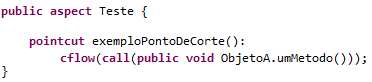
\includegraphics{img/flow_p1.png}
	\caption{Ponto de corte para captura do fluxo de execução inclusivo: cflow()}\label{fig:flow_p1}
\end{figure}

\begin{figure}[!hb]
	\centering
	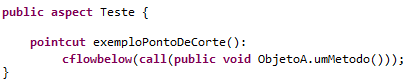
\includegraphics{img/flow_p2.png}
	\caption{Ponto de corte para captura do fluxo de execução exclusivo: cflowbelow()}\label{fig:flow_p2}
\end{figure}
 
Além dos pontos de corte para captura de execução, chamada, tratamento de exceção e atribuição, existem pontos de corte mais complexos relativos ao
fluxo de execução de um programa. Os \textbf{pontos de corte para captura do fluxo de execução} capturam todos os pontos de junção a partir de um outro ponto de
corte. Existem dois tipos: \textit{cflow(PontoDeCorte)} e \textit{cflowbelow(PontoDeCorte)}. O ponto de corte da figura \ref{fig:flow_p1}
é do tipo \textit{cflow()} e captura todos os pontos de junção disparados a partir do ponto de corte \textbf{call(public void ObjetoA.umMetodo())},
inclusive a chamada ao próprio método. O ponto de corte da figura \ref{fig:flow_p2} é do tipo \textit{cflowbelow()} e captura os mesmos pontos de
junção do anterior, exceto a chamada ao próprio método.

\begin{landscape}
\begin{figure*}
	\centering
	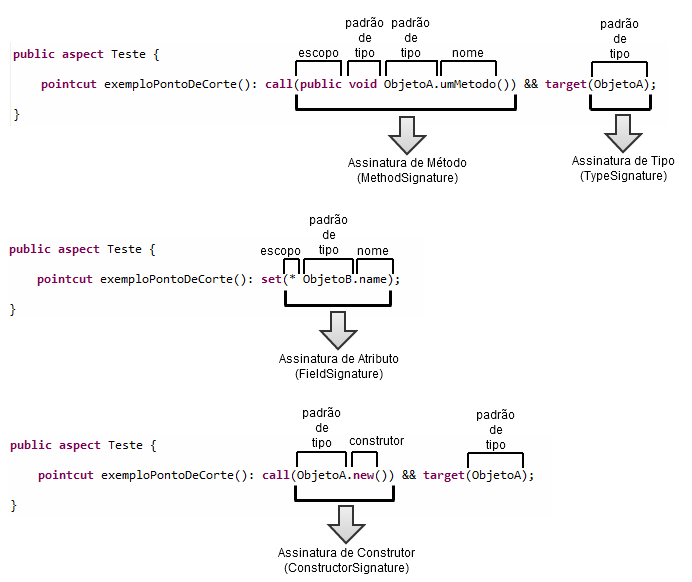
\includegraphics[scale=0.8]{img/signatures.png}
	\caption{Exemplo de assinaturas em AspectJ}\label{fig:signatures}
\end{figure*}
\end{landscape}

Existem também \textbf{pontos de corte baseados na estrutura léxica do código}. Estes pontos de corte capturam pontos de junção que ocorrem dentro de
um determinado trecho de código. Existem dois tipos: \textit{within(AssinaturaDeTipo)} e \textit{withincode(AssinaturaDeConstrutor ou
AssinaturaDeMétodo)}. O primeiro tipo captura os pontos de junção que ocorrerem dentro de classes, aspectos ou classes aninhadas de um determinado
tipo (\textit{AssinaturaDeTipo}. O segundo tipo captura os pontos de junção que estiverem dentro do código de um dado método ou construtor
(\textit{AssinaturaDeConstrutor ou AssinaturaDeMetodo}). 

Outros tipos de \textbf{ponto de corte permitem capturar o contexto de uma
execução}. O ponto de corte \textit{this(TipoDoObjeto)} permite capturar todos
os pontos de junção onde o objeto que está executando é do tipo
\textit{TipoDoObjeto}. Já o ponto de corte \textit{target(TipoDoObjeto)} permite
capturas os pontos de junção onde o objeto que está sendo chamado é do tipo
\textit{TipoDoObjeto}. Estes pontos de corte permitem passar o contexto de uma execução, isto é, instâncias de objetos, para um aviso,
o que será abordado ainda neste capítulo. 

Existem também os \textbf{pontos de corte para argumentos}.
Estes pontos de corte tem a seguinte sintaxe: \textit{args(AssinaturaDeTipo, 
\ldots , AssinaturaDeTipo)}. Eles permitem capturar pontos de junção
baseados nos argumentos recebidos. Por exemplo, capturar os métodos 
que recebam três atributos do tipo \textit{String}.

Após identificar quais pontos de junção serão capturados através de pontos de
corte, deve-se especificar qual o comportamento que será executado antes, 
durante ou depois dos locais selecionados. Para isso, AspectJ propõe uma
construção denominada \textbf{aviso}. Um aviso é uma construção parecida com um método
em Java. Ele define um comportamento para ser executado. Existem três tipos de
avisos:

\begin{itemize}
  \item \textbf{Antes} (before): Executa antes do ponto de junção capturado.
  \item \textbf{Depois} (after): Executa depois do ponto de junção capturado.
  Existe uma variação ao aviso \textit{after} que executará apenas se o ponto de
  junção capturado não lançar nenhuma exceção, isto é, só será executado se a execução
  do ponto de junção tiver sucesso. Esse tipo de aviso é denominado
  \textit{after returning}.
  \item \textbf{Durante} (around): É o tipo de aviso mais poderoso, pois
  pode executar no lugar do ponto de junção capturado, continuar a execução
  original ou alterar o contexto de execução.
\end{itemize}

A figura \ref{fig:advice_code} mostra um exemplo de um aviso que executa
\textbf{depois}(\textit{after}) do ponto de corte
\textbf{exemploDePontoDeCorte()}. Este aviso recebe o contexto da execução
como parâmetro (um objeto do tipo \textbf{ObjetoA}) e imprime uma
mensagem com a representação textual deste objeto. O corpo deste aviso é o
trecho de código que realiza a impressão da representação do objeto. Em AspectJ,
o corpo de um aviso pode conter qualquer código Java. Observa-se também que o
objeto passado no contexto de execução é referenciado no corpo do aviso. Os
pontos de corte \textit{target()} e \textit{this()} são muito utilizados, pois
permitem passar o contexto de execução para um aviso.

\begin{figure}[!hb]
	\centering
	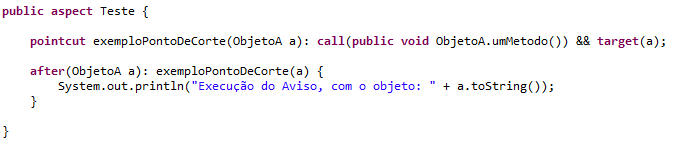
\includegraphics{img/advice_code.png}
	\caption{Exemplo de aviso com contexto de execução}\label{fig:advice_code}
\end{figure}

\subsubsection{Construções Estáticas}

Uma das construções estáticas propostas por AspectJ é a \textbf{introdução}, que
permite alterar a estrutura de classes, aspectos e interfaces adicionando novos
métodos e atributos. A figura \ref{fig:introduction} mostra um aspecto que
introduz o método \textbf{metodoIntroduzido()} e os atributos
\textbf{atributoUm} e \textbf{atributoDois} na classe do tipo \textbf{ObjetoA}.
Os dois atributos introduzidos são utilizados no próprio método
\textbf{metodoIntroduzido()}. Isto é possível, pois
o compilador AspectJ sabe que o método introduzido pertence ao \textbf{ObjetoA}
e o objeto que executará este método será um objeto do tipo \textbf{ObjetoA}.

\begin{figure}
	\centering
	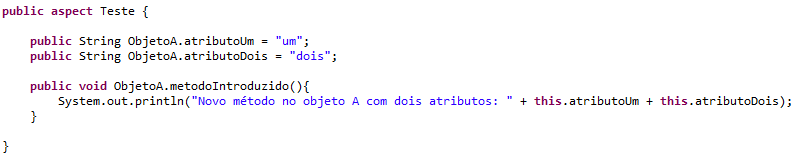
\includegraphics{img/introduction.png}
	\caption{Introdução de métodos e atributos}\label{fig:introduction}
\end{figure}

Outra funcionalidade disponível na linguagem é a \textbf{modificação da hierarquia de classes}, permitindo a definição de
relacionamentos de herança, implementação de interfaces, dentre outras
alterações \cite{Laddad:2003:AAP:993468}. O exemplo da figura
\ref{fig:introduction_interface} mostra a introdução de um relacionamento de
herança entre as classes \textbf{ObjetoA} e \textbf{ObjetoB}.

\begin{figure}
	\centering
	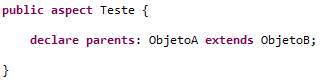
\includegraphics{img/introduction_interface.png}
	\caption{Introdução de relacionamentos de herança}\label{fig:introduction_interface}
\end{figure}

\subsubsection{Aspecto}

Resumidamente, para estender um sistema utilizando Java com AspectJ, deve-se
identificar os pontos de junção que serão selecionados por um ponto de corte e
implementar o aviso que introduzirá o novo comportamento antes, durante ou
depois do ponto de corte. O elemento da linguagem que agrupa todas essas
construções é o \textbf{aspecto}. Um aspecto é uma unidade de modularização 
semelhante a uma classe, mas com diferenças em relação ao ciclo de vida, pois
não pode ser instancializado e não pode especializar de um outro aspecto concreto.
No entanto, um aspecto pode ser declarado como abstrato e aspectos concretos
podem estendê-lo para implementar suas declarações abstratas.

\subsubsection{Exemplo de Aspecto}

O objetivo deste exemplo é utilizar a linguagem AspectJ para implementar de maneira elegante o padrão de projeto \textbf{Observador}
\cite{Gamma:1995:DPE:186897}. Este padrão permite que um ou mais objetos se cadastrem para escutar mudanças de um outro objeto. A implementação do padrão está 
presente nos exemplos da IDE para desenvolvimento com aspectos: AspectJ Development Tools (AJDT) \cite{AspectJ11}.

Um dos requisitos deste padrão é que um ou mais objetos (observadores) possam
escutar mudanças de um outro objeto (sujeito) e serem atualizados. Assim,
identificam-se duas interfaces: \textit{Subject} e \textit{Observer}. A interface \textit{Subject}
deve armazenar seus observadores e prover métodos para adicionar, remover e obter
os mesmos. A interface \textit{Observer} deve prover métodos para associar e
obter o sujeito observado. Esses requisitos são implementados no aspecto como
introduções de métodos e atributos. O trecho de código da figura \ref{fig:aspects_observer_1} apresenta as introduções realizadas. Observa-se a
introdução do atributo \textit{observers} e dos métodos \textit{addObserver()},
\textit{removeObserver()} e \textit{getObservers()} na interface
\textit{Subject}. Na interface \textit{Observer} foram introduzidos os métodos
\textit{setSubject()} e \textit{getSubject()} e o atributo
\textit{subject}.

Além de introduzir os métodos e atributos para permitir a associação entre
sujeitos e observadores, deve-se implementar a lógica que capture mudanças nos
sujeitos e avise os observadores. Essa lógica pode ser implementada com o uso de
pontos de corte e avisos. O ponto de corte \textit{stateChanges()} é
responsável por escutar mudanças em um sujeito e após (\textit{after}) cada
mudança, um aviso é executado para atualizar os observadores. O ponto de corte
\textit{stateChanges()} deve ser abstrato, pois este ponto de corte será
diferente para cada sujeito a ser observado. O trecho de código que implementa o
ponto de corte e o aviso também pode ser visualizado na figura \ref{fig:aspects_observer_1}.

Com esses requisitos implementados, é possível juntar os dois trechos de código
em um aspecto abstrato que implementa o padrão \textbf{Observador}. Este aspecto
é abstrato, pois tem o ponto de corte abstrato \textit{stateChanges()}, que deve
ser definido por um aspecto concreto, selecionando quais pontos de junção serão
capturados para definir que uma mudança ocorreu. O aspecto abstrato recebe o
nome de \textit{SubjectObserverProtocol} e pode ser visualizado na figura
\ref{fig:aspects_observer_1}. Um desenvolvedor que deseja utilizar o padrão de projeto
observador pode reusar o aspecto abstrato \textit{SubjectObserverProtocol}, 
estendendo-o com a implementação de um aspecto concreto. Este aspecto concreto
deve especificar qual classe faz o papel de sujeito, isto é, qual classe
implementa a interface \textit{Subject} e qual classe faz o papel de
observador, isto é, qual classe implementa a interface \textit{Observer}.
Além disso, deve definir o ponto de corte \textit{stateChanges()}, para
especificar em quais pontos de junção serão detectadas mudanças. 

\begin{figure}
	\centering
	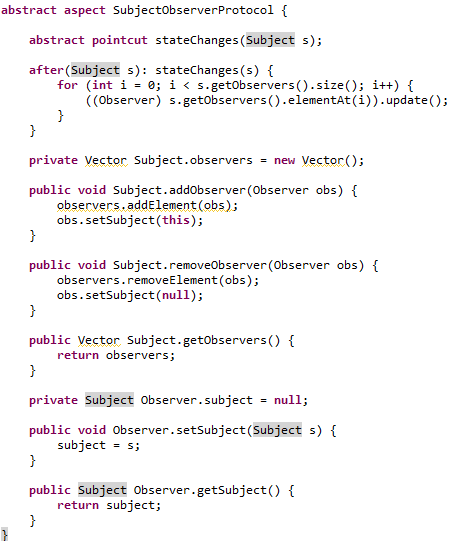
\includegraphics{img/aspects_observer_1.png}
	\caption{Aspecto abstrato para implementação do padrão de projeto Observador}\label{fig:aspects_observer_1}
\end{figure}

Considerando como exemplo um sistema de interface gráfica com um botão e um
texto com cor variável. Define-se como requisito que a cor deste texto deve modificar toda vez
que o botão foi clicado. Este requisito pode ser implementado utilizando o
aspecto abstrato. O pequeno sistema de interface gráfica contém a classe
\textit{Button} representando o botão e a classe \textit{ColorLabel}
representando o texto com cor. A classe \textit{Button} é o sujeito observado,
por isso implementa a interface \textit{Subject}. O observador é a classe
\textit{ColorLabel} que implementa a interface \textit{Observer}. Além disso,
introduz-se o método \textit{update()} na classe \textit{ColorLabel} para
atualizar a cor do texto quando houver alguma mudança no botão. O que está
faltando definir é quais pontos na execução do programa geram mudanças no botão.
Estes pontos são definidos ao implementar o ponto de corte abstrato
\textit{stateChanges()}. Define-se que serão capturadas as chamadas ao método
\textit{click()} da classe \textit{Button}, onde o objeto alvo é do tipo
\textit{Subject} (neste caso é da classe \textit{Button}, pois esta classe
implementa \textit{Subject}. O código do aspecto concreto para implementar o
padrão observador pode ser visualizado na figura \ref{fig:aspects_observer_2}. 
Este aspecto captura cliques em um botão, atualizando a cor de um texto.

\begin{figure}
	\centering
	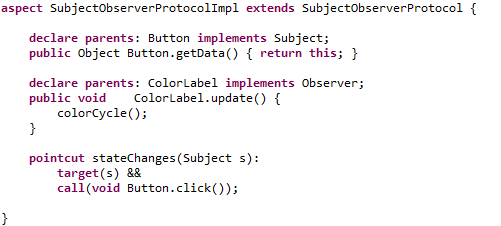
\includegraphics{img/aspects_observer_2.png}
	\caption{Aspecto concreto implementando o padrão de projeto Observador em um sistema de
	interface gráfica}\label{fig:aspects_observer_2}
\end{figure}

\section{Análise e Projeto com UML}

A análise e projeto de sistemas orientados a objetos é uma abordagem utiliza no desenvolvimento de aplicações complexas. 
Aplicações complexas necessitam de um planejamento antes da implementação. Usualmente divide-se o desenvolvimento de
um sistema em quatro fases: análise, projeto, implementação e testes
\cite{pressman:01}. As fases de análise e projeto são as fases aonde realiza-se 
a maior parte do planejamento de um desenvolvimento. Já as fases de
implementação e testes são responsáveis pela codificação com o objetivo de obter
um programa executável e que cumpra os requisitos do cliente. 

Nas fases de análise e projeto utilizam-se modelos que permitem representar o
sistema em diferentes níveis de abstração, facilitando a compreensão e reduzindo
a complexidade. A fase de análise tem como objetivo compreender os principais conceitos
do domínio do problema, evitando o uso de termos computacionais. Já a fase de
projeto foca na solução que será desenvolvida para produzir um sistema a partir
da compreensão do problema. 

\subsection{Múltiplos pontos de vista de um sistema}

Segundo \cite{silva:07}, um sistema orientado a objetos pode ser visualizado por
diferentes pontos de vista:

\begin{itemize}
  \item Estrutural de sistema: Essa visão contém o conjunto de elementos de um
  sistema orientado a objetos e seus relacionamentos.
  \item Estrutural de classe: Essa visão contém o detalhamento da estrutura de
  cada um dos elementos de um sistema.
  \item Comportamental de sistema: Essa visão permite compreender o
  conjunto de funcionalidades do sistema e como os elementos iteragem em tempo
  de execução.
  \item Comportamental de classe: Essa visão permite compreender o comportamento
  de um elemento isoladamente. Geralmente compreende-se a variação de estados
  desse elemento.
\end{itemize}
  
Uma modelagem que permita representar esses quatro pontos de vista pode ser considerada completa. Uma \textbf{modelagem completa} fornece subsídios
para a geração de código e facilita a compreensão e manutenção de um sistema. 

\section{UML: Segunda Versão}

A segunda versão da UML \cite{uml:05} permite representar o comportamento e a estrutura de um sistema nas fases de análise e projeto
através de diagramas estruturais e comportamentais. Esta linguagem é um padrão da \textit{Object Management Group} (OMG)\sigla{OMG}{Object Management
Group}, por isso é compreendida e utilizada por grande parte dos desenvolvedores e analistas para realizar a modelagem de sistemas. Os
diagramas da segunda versão da UML permitem a representação dos quatro pontos de vista essenciais para programas  orientados a objetos. As seções que tratam dos diagramas estruturais e
comportamentais da UML são baseadas no conteúdo do livro UML 2 em Modelagem Orientada a Objetos \cite{uml2ricardo:03} e no Tutorial de UML da Sparx
Systems \cite{sparx_tutorial}.

\subsection{Diagramas Estruturais}

A segunda versão da UML disponibiliza sete diagramas estruturais: diagrama de classes, componentes, estrutura composta, instalação, objetos,
pacotes e perfil. Os diagramas estruturais utilizados nesta dissertação são os diagramas de classe e o diagrama de perfil. Este último foi
introduzido na versão 2.2 da linguagem e é utilizado para a extensão da linguagem para um domínio específico.

\subsubsection{Diagrama de Classes}

O diagrama de classes permite representar a estrutura e os relacionamentos dos elementos de um sistema. Este diagrama permite visualizar o sistema
como um todo, visualizando os relacionamentos entre os elementos e também permite visualizar a estrutura de cada elemento, com seus atributos e
métodos. Os principais componentes deste diagrama são as classes, associações, atributos, métodos e pacotes.

\subsubsection{Diagrama de Perfil}

O diagrama de perfil permite estender o modelo da linguagem para representar conceitos de um determinado domínio de aplicações. Um perfil é composto
por \textbf{estereótipos}, \textbf{restrições} e \textbf{valores rotulados}. 

Um \textbf{estereótipo} adiciona uma semântica adicional a um elemento da UML. Geralmente adiciona-se um estereótipo para diferenciar os papéis dos
elementos de um modelo. Por exemplo, a classe \textit{RoomManager} da figura \ref{fig:stereotype_1} foi associada ao estereótipo \textit{Controller} 
para representar que esta classe tem o papel de controlador. É possível adicionar mais de um estereótipo a mesma classe. A classe
\textit{ReservationManager} é associada aos estereótipos \textit{Controller} e \textit{Client} para representar que esta classe é
um controlador e que encontra-se do lado do cliente. Os estereótipos \textit{Client} e \textit{Controller} estendem o elemento do 
meta-modelo da UML \textit{Class}, podendo assim ser aplicados a qualquer classe.  É importante observar que um estereótipo pode ser associado a
qualquer elemento do meta-modelo da UML. O atributo \textit{id} da classe \textit{Room} está associado ao estereótipo \textit{key} para representar
que este atributo define unicamente uma sala. O estereótipo \textit{key} está estendendo o meta-modelo da UML \textit{Attribute}.

\begin{figure}
	\centering
	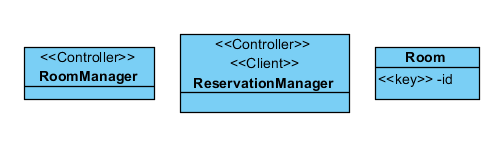
\includegraphics[scale=0.9]{img/stereotype_1.png}
	\caption{Uso de estereótipos em um diagrama de classes}\label{fig:stereotype_1}
\end{figure}

Um estereótipo adiciona um papel a um elemento do modelo. Para adicionar mais informações a um elemento, podem-se definir \textbf{valores rotulados}.
A linguagem permite associar zero ou mais valores rotulados a um estereótipo. Um valor rotulado pode ser um elemento do modelo, um número, um texto, um booleano ou uma 
enumeração definida pelo usuário. Ao utilizar um estereótipo em um modelo, deve-se definir os valores rotulados associados ao mesmo. Os valores
rotulados adicionam uma semântica ao estereótipo. O exemplo da figura \ref{fig:tagged_values_1} contém duas classes que representam sistemas
operacionais: \textit{Fedora64} e \textit{WindowsXP}. Estas classes são marcadas com o estereótipo \textit{Operating System}. Este estereótipo 
exige a definição do valor rotulado \textit{platfom}, que define qual a plataforma do sistema operacional. Este valor rotulado é um enumerado com dois
tipos: x86 e x64. No exemplo, a classe \textit{Fedora64} associa o valor x64 ao valor rotulado \textit{platform}, pois é um sistema de 64 bits. Já a classe
\textit{WindowsXP} associa o valor x86 ao mesmo valor rotulado, pois é um sistema de 32 bits. Finalmente, \textbf{restrições} podem ser
introduzidas ao modelo para garantir a consistência no próprio modelo e nos seus relacionamentos.

\begin{figure}
	\centering
	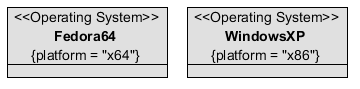
\includegraphics{img/tagged_values_1.png}
	\caption{Uso de valores rotulados em um diagrama de classes}\label{fig:tagged_values_1}
\end{figure}

A figura \ref{fig:profile_diagram} mostra a definição de um perfil UML para modelagem de sistemas que desejam representar veículos
\cite{VisualParadigm11}. Foram definidos sete estereótipos que estendem o elemento do meta-modelo \textit{Class}. Observa-se a generalização entre os
estereótipos \textit{Vehicle}, \textit{Mini}, \textit{Pickup Truck} e \textit{Convertible}. O estereótipo \textit{Pickup Truck} especializa o
estereótipo \textit{Vehicle}. O relacionamento de composição entre os estereótipos \textit{Interior} e \textit{Seat} define que o interior de um
veículo deve ter no mínimo um assento. Observa-se também a presença de dois valores rotulados do tipo texto no estereótipo \textit{Seat}:
\textit{texture} e \textit{pattern}. Existem outros valores rotulados neste perfil como: o limite de passageiros (\textit{passenger-limit}) no
estereótipo \textit{Vehicle}, que é do tipo inteiro; o limite de velocidade (\textit{speed-limit}) também no estereótipo \textit{Vehicle}, que é do
tipo ponto flutuante, dentre outros. Este perfil pode ser exportado no formato \textit{XML Metadata Interchange} (XMI)\sigla{XMI}{XML Metadata Interchange} \cite{xmi:11} 
e utilizado por outras ferramentas do tipo \textit{Computer Aided Software Engineering} (CASE)\sigla{CASE}{Computer Aided Software Engineering}. Assim, 
é possível intercambiar perfis entre diferentes ferramentas CASE. A vantagem do intercâmbio de perfis é o reuso de
especificações já prontas sobre um determinado domínio de aplicação. Um exemplo de perfil que pode ser reusado por outros desenvolvedores é um perfil
que especifique sistemas orientados a aspectos.

\begin{landscape}
\begin{figure*}
	\centering
	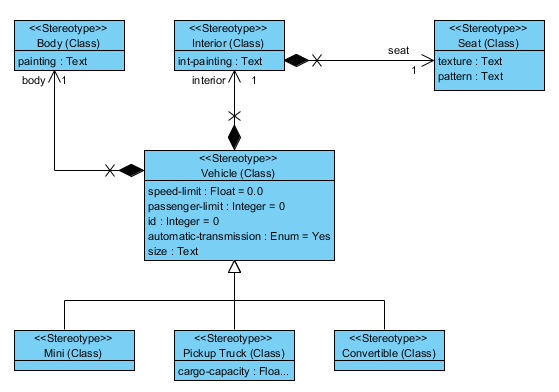
\includegraphics{img/profile_diagram.png}
	\caption{Diagrama de Perfil para representar veículos}\label{fig:profile_diagram}
\end{figure*}
\end{landscape}

\subsection{Diagramas Comportamentais}

A segunda versão da UML possui sete diagramas comportamentais: diagrama de atividades, máquina de estados, casos de uso, comunicação, visão geral de 
interação, sequência e de tempo. Neste trabalho serão utilizados os diagramas de máquina de estados e de sequência.

\subsubsection{Diagrama de Máquina de Estados}

O diagrama de máquina de estados representa os estados e o comportamento de um objeto, especificando a sequência de eventos que um objeto recebe
durante sua existência. Os principais componentes deste diagrama são os estados e as transições. Um diagrama de máquina de estados também pode
representar concorrência utilizando nodos \textit{fork} e \textit{join} com regiões concorrentes. Este mecanismo permite realizar a sincronização
entre diferentes estados. Na POO utiliza-se o diagrama de máquina de estados para especificar os diferentes estados de uma classe.
Neste caso, cada estado representa uma configuração dos atributos da classe. As transições são as execuções de métodos, que modificam valores de
atributos, evoluindo a classe para um novo estado.

\subsubsection{Diagrama de Sequência}

O diagrama de sequência representa as trocas de mensagens entre objetos. Este diagrama permite compreender a interação entre objetos com
foco no tempo e na ordem das mensagens durante uma execução. Os principais componentes do diagrama de sequência são as linhas de vida de objetos, as
mensagens e os fragmentos combinados. Um fragmento combinado permite adicionar condições e iterações em uma troca de mensagens. Outro componente
utilizado nesta dissertação é a invariante de estado, que permite estabelecer uma condição para que um conjunto de mensagens seja executado. Este conjunto de mensagens somente será executado quando o sistema atingir o estado associado com a invariante de estado. O comportamento
de cada caso de uso pode ser refinado com um diagrama de sequência.

\section{Model-Driven Engineering}

O aumento da complexidade das plataformas mais utilizadas no desenvolvimento de software (CORBA, J2EE, .NET) gera um grande esforço para
desenvolvedores portarem código de aplicação para estas plataformas \cite{Schmidt:2006:GEI:1115688.1115706}. A manutenção do código das aplicações e
das plataformas ainda é realizada utilizando linguagens de programação tradicionais, como Java e C++. A complexidade destas plataformas implementadas
com linguagens tradicionais dificulta a obtenção de uma visão unificada, que facilite a compreensão do impacto de uma mudança no sistema.

Model-Driven Engineering (MDE) \sigla{MDE}{Model-Driven Engineering} é uma metodologia de desenvolvimento de software focada na representação de
elementos de um domínio de problema em nível de modelo. Esta metodologia surgiu com o objetivo de permitir uma melhor representação destas plataformas
complexas. A técnica de MDE utiliza meta-modelagem para representar o domínio de uma aplicação, definindo os relacionamentos entre os conceitos do
sistema. Através da meta-modelagem, define-se uma linguagem específica para um determinado domínio, que pode ser reusada. A partir desta linguagem,
independente de plataforma, é possível utilizar um transformador que transforma os modelos em uma linguagem alvo.

A metodologia de MDE tem um futuro promissor, pois permite diminuir a complexidade na representação de conceitos de um domínio de aplicação
ou de uma plataforma. A linha de aprendizado de um sistema modelado com a técnica de MDE é menor do que com modelagem tradicional (somente UML) ou com
linguagens tradicionais. A manutenabilidade do sistema também é facilitada utilizando MDE.

\section{Meta-modelagem}

Uma linguagem geralmente é definida através de uma gramática na forma \textit{Backus Naur Form} (BNF) \sigla{BNF}{Backus Naur Form}. Uma linguagem
bem definida pode ser interpretada de forma automatizada por um computador. Este método de definição de linguagens é utilizado até hoje para
representar linguagens baseadas em texto. Para facilitar a definição de linguagens para modelagem pode-se utilizar um outro mecanismo. Este mecanismo
é denominado \textbf{meta-modelagem}, que permite a descrição de uma linguagem na forma de um modelo \cite{mda:03}. Um meta-modelo de uma linguagem define os 
elementos que podem ser utilizados na criação de modelos utilizando esta linguagem. Considerando a UML como exemplo, o meta-modelo da linguagem define
elementos como Classe, Estado, Pacote, Operação, etc. Assim, um modelo definido utilizando UML pode definir instâncias de classes, estados, pacotes, operações, etc. 
A OMG define uma arquitetura em quatro camadas para representar os modelos padrões para definição de modelos. Esta arquitetura pode ser visualizada
na figura \ref{fig:omg_meta_model}. 

Na arquitetura da figura \ref{fig:omg_meta_model}, o modelo M3 define elementos que podem ser utilizados para representar conceitos no modelo M2. O
modelo M3 é considerado o meta-meta-modelo da OMG. O \textit{Meta-Object Facility} (MOF) \sigla{MOF}{Meta-Object Facility}) é um padrão da OMG que define a linguagem que
deve ser utilizada para definir linguagens para modelagem \cite{mof:11}. O MOF está no nível M3. O modelo M2 especifica os elementos que podem ser
utilizados no modelo M1. Um modelo no nível M2 é denominado um meta-modelo. Linguagens geralmente são definidas neste nível de modelo. Observa-se na
figura \ref{fig:omg_meta_model} a definição de uma classe (\textit{UML Class}) e de um atributo (\textit{UML Attribute}) no nível M2. Estes elementos
fazem parte da definição do meta-modelo da UML. O modelo M1 contém instâncias de elementos definidos no modelo M2. Este modelo é o que é definido
pelo analista ao realizar a modelagem de um determinado sistema com UML. Na figura \ref{fig:omg_meta_model} observa-se a definição de duas classes:
\textit{Customer} e \textit{Order} no nível M1. Além disso, definem-se os atributos \textit{title}, \textit{name} e \textit{number} nessas classes. As
classes são instâncias da meta-classe \textit{UML Class}. Os atributos são instâncias da meta-classe \textit{UML Attribute}. Finalmente, o modelo M0
representa as instâncias de um sistema representadas em um modelo. Um exemplo de instância é um cliente do tipo \textit{Customer} com o nome
\textit{Joe Nobody}.

\begin{figure}
	\centering
	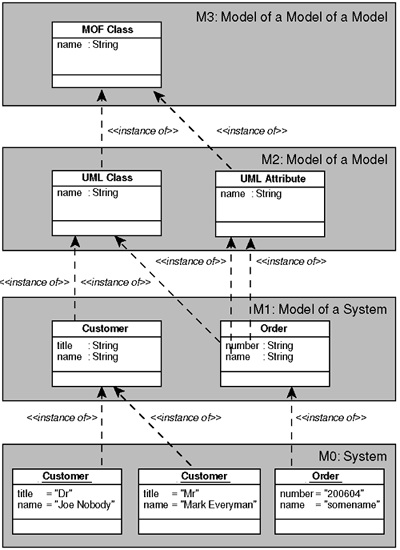
\includegraphics{img/omg_meta_model.png}
	\caption{Meta-modelo da Object Management Group (OMG)}\label{fig:omg_meta_model}
\end{figure}

O meta-modelo da UML é definido no nível M2 a partir do MOF. Este meta-modelo é uma instância do MOF. Uma parte do meta-modelo pode ser visualizada na
figura \ref{fig:uml_meta_model}. Esta parte do modelo define os componenentes para representar classes, atributos, operações, etc.

\begin{figure}
	\centering
	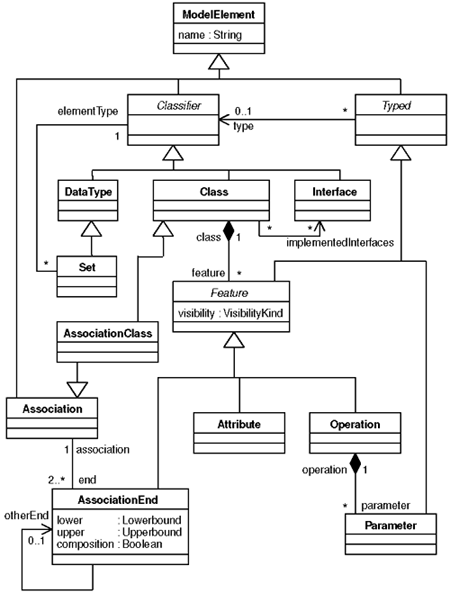
\includegraphics{img/uml_meta_model.png}
	\caption{Meta-modelo da UML}\label{fig:uml_meta_model}
\end{figure}

É importante observar no modelo da figura \ref{fig:uml_meta_model} que qualquer elemento de um modelo da UML deve derivar de \textit{ModelElement} e
por isso deve ter um nome. Nota-se também a presença de Classe (\textit{Class}), Atributo (\textit{Attribute}) e Operação (\textit{Operation}). Estes
são alguns dos elementos que podem ser utilizados na criação de uma modelagem utilizando UML. Os relacionamentos entre os elementos do meta-modelo
podem introduzir restrições. Um exemplo de restrição é que uma operação pode ter zero ou mais parâmetros. Qualquer modelo da UML deve respeitar estas
restrições e a estrutura definida no meta-modelo da OMG.

\subsection{Extensões a UML}

É possível estender a UML de duas formas: criação de um Perfil UML para representar os conceitos de um dado domínio de aplicação ou através da
definição de um novo meta-modelo para este domínio de aplicação.

\subsubsection{Extensão pela Definição de um Perfil UML}

A UML pode ser estendida com a definição de diferentes perfis para determinados domínios de aplicação. É importante observar que, o mecanismo de
perfis não é um mecanismo de extensão de primeira classe, o que significa que um perfil não pode modificar um meta-modelo (removendo restrições da
UML, por exemplo), apenas adaptá-lo com construções específicas do domínio tratado. O mecanismo de extensão por perfis é considerado uma mecanismo
leve para extensão da linguagem.

A grande vantagem de estender a UML através de perfis é que qualquer ferramenta que suporte a importação de perfis pode utilizar os conceitos
estendidos pelo perfil UML. Como o diagrama de perfil é um padrão da UML, a maior parte das ferramentas CASE já está suportando a definição e
importação de perfis. Outra vantagem deste mecanismo é que é possível aplicar mais de um perfil em um mesmo modelo. Além disso um Perfil UML pode ser
facilmente modificado, com a introdução de novos estereótipos, valores rotulados e restrições. Esta modificação pode ser realizada em qualquer ferramenta 
CASE que suporte a importação e definição de perfis.

\subsubsection{Extensão pela Definição de um Meta-modelo}

Com meta-modelagem, o objetivo é estender o meta-modelo da UML no nível M2 com a adição de novos conceitos relacionados a um domínio de aplicação. Uma
extensão neste nível modifica o meta-modelo, podendo adicionar e remover restrições, adicionar e remover meta-classes do modelo, adicionar e
modificar relacionamentos, etc. 

Este tipo de extensão não permite o reuso dos conceitos em qualquer ferramenta de modelagem, pois as ferramentas CASE suportam apenas a definição de
modelos dentro do meta-modelo padrão da OMG ou modelos definidos com o uso de de perfis. Assim, a extensão será específica para uma determinada
ferramenta. A extensão através de meta-modelagem pode ser utilizada quando uma extensão tem uma baixa probabilidade de ser modificada no futuro e não
existe a necessidade de combinar esta extensão com outras extensões.

